\section{Morphological Image Processing\buch{Ch. 9}}
\subsection{Set Theory}
\subsubsection{Reflection}
\[
	\hat{B} = \{w | w = -b,\quad \text{for} \quad b \in B \}
\]


\subsubsection{Translation}
\[
	(B)_z = \{ c | c = b + z,\quad \text{for} \quad b \in B\}
\]


\subsubsection{Erosion}
With A and B as sets in $Z^2$, the erosion of A by B is defined as
\[
	A \ominus B = \{z|(B)_z \subseteq A  \}
\]

This is the set of all translations by z such that the set B is still a subset of A.

Equivalently, if B must be contained in A, it is not allowed to intersect with the background:
\[
	A \ominus B = \{z|(B)_z \cap A^c = \varnothing  \}
\]


\subsubsection{Dilation}
With A and B as sets in $Z^2$, the dilation of A by B is defined as
\[
	A \oplus B = \{z |(\hat{B})_z \cap A \neq \varnothing \}
\]
This is the set of all translations by z such that the set B reflected about its origin has at leas one overlap with the set A.

Equivalently, since the intersection is not allowed to be empty and all elements in it must be from A:
\[
	A \oplus B = \{z | [(\hat{B})_z \cap A] \subseteq A \}
\]


\subsubsection{Duality erosion/dilation}
Erosion and dilation are dual:
\[
	(A  \ominus B)^c = A^c \oplus \hat{B}
\]
\[
	(A \oplus B)^c = A^c \ominus \hat{B}
\]


\subsubsection{Opening and closing}
The opening of A by B is defined: (first erosion then dilation)
\[
	A \circ B = (A \ominus B) \oplus B
\]

The closing of A by B is defined: (first dilation then erosion)
\[
	A  \bullet B = (A \oplus B) \ominus B
\]

Opening and closing are dual operations: 
\[
	(A  \bullet B)^c = (A^c \circ \hat{B})
\]
\[
	(A \circ B)^c = (A^c \bullet \hat{B})
\]

\begin{figure}
	\centering
	\begin{subfigure}[b]{0.45\textwidth}
		\centering
		\adjustbox{scale=0.5}{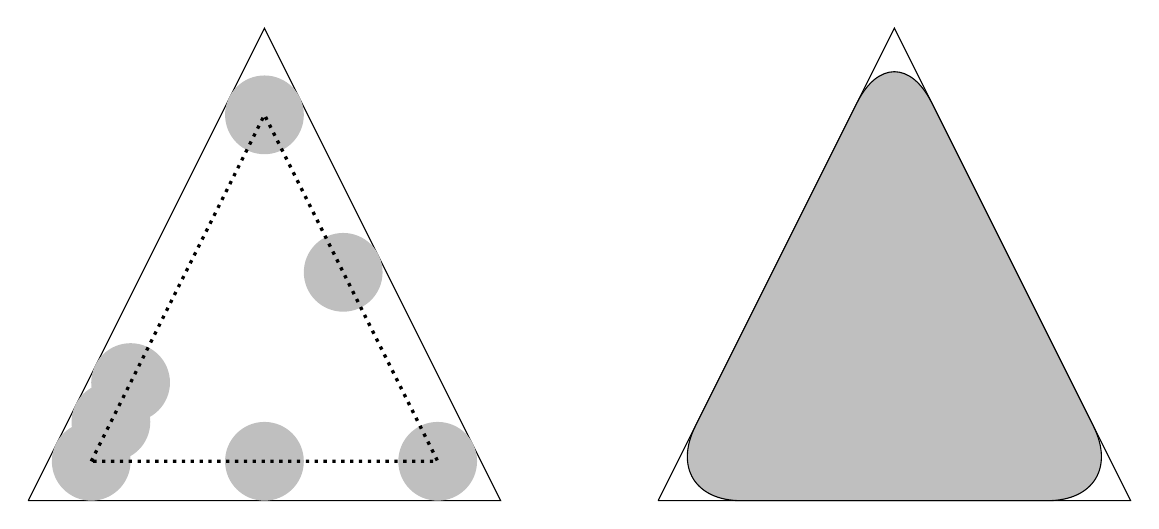
\begin{tikzpicture}
%linkes dreieck
\draw (0,0) -- (3,6) -- (6,0) -- (0,0);
\fill [lightgray] (0.8,0.5) circle (0.5);
\fill [lightgray] (1.05,1) circle (0.5);
\fill [lightgray] (1.3,1.5) circle (0.5);
\fill [lightgray] (3,4.9) circle (0.5);
\fill [lightgray] (4,2.9) circle (0.5);
\fill [lightgray] (5.2,0.5) circle (0.5);
\fill [lightgray] (3,0.5) circle (0.5);
\draw [dotted, very thick] (0.8,0.5) -- (3,4.9) -- (5.2,0.5) -- (0.8,0.5);

\draw (8,0) -- (11,6) -- (14,0) -- (8,0);
\draw [rounded corners=30pt, fill=lightgray] (9,2) -- (11,6) -- (14,0) -- (8,0) -- (9,2);

\end{tikzpicture}}
		\caption{Opening}
	\end{subfigure}
	\begin{subfigure}[b]{0.45\textwidth}
		\centering
		\adjustbox{scale=0.5}{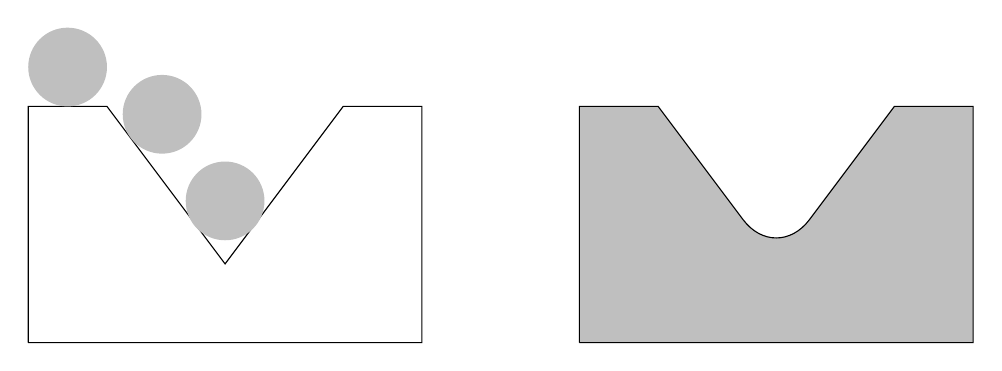
\begin{tikzpicture}

\draw (0,0) -- (0,3) -- (1,3) -- (2.5,1) -- (4,3) -- (5,3) -- (5,0) -- (0,0);
\fill [lightgray] (0.5,3.5) circle (0.5);
\fill [lightgray] (1.7,2.9) circle (0.5);
\fill [lightgray] (2.5,1.8) circle (0.5);

\draw [fill=lightgray] (7,0) -- (7,3) -- (8,3) [rounded corners=20pt] -- (9.5,1) [rounded corners=0] -- (11,3) -- (12,3) -- (12,0) -- (7,0);

\end{tikzpicture}}
		\caption{Closing}
	\end{subfigure}
	\caption{Geometrical interpretation of the opening and closing transformations}
\end{figure}


\subsubsection{The hit-or-miss transform}
The hit-or-miss transform is a basic tool for shape detection. Basic idea:
\begin{itemize}
	\item Through erosion of the image by the object, possible locations for the object in the image are left, since elements smaller than the objects disappear
	
	\item Through erosion of the background of the image with the local background of the object, possible locations for the object in the image are left
	
	\item The intersection of these possible locations result in a reliable  detection of the object location
	\[
		A \circledast B = (A \ominus D) \cap [ A^c \ominus (W-D)]
	\]
	
	\item In general, if B1 is the object and B2 is the corresponding background this can be written
	\[
		A \circledast B = (A \ominus B_1)\cap (A^c \ominus B_2)	
	\]	
\end{itemize}

\subsection{Some basic morphological algorithms}
\subsubsection{Convex hull}
\begin{itemize}
\item The convex hull H of a set S is the smalles convex set containing S.
\item H-S is called the convex deficiency of S
\end{itemize}
The convex hull is constructed with a convex hull with four structuring elements.
%TODO Image page 26
The resulting set is not the smallest convex set that contains A. The following additional constraints can be used:
\begin{itemize}
\item The convex hull is not allowed to grow beyond the original vertical and horizontal dimension
\item 
\end{itemize}

\subsubsection{Thinning}
Thinning is the operation of making the foreground thinner.
%TODO Image page 29
	\[
		A \otimes  B = A - (A \circledast B)	
	\]	
Hit or miss transformation with rotating structuring elements.\\

%TODO Image 8 structuring elements page 31
	\[
		A \otimes  {B} = ((\ldots((A \otimes B^{1}) \otimes B^{2})\ldots) \otimes B^{n})	
	\]	

\subsubsection{Thickening}
This is the morphological dual of thinning. It is implemented as thinning the background and then taking the complement.

\subsubsection{Skeleton S(A)}
%TODO Image page 33
Finding a disk D that:
\begin{itemize}
\item centers at z
\item there is no larger disk containing D and included in A
\item touches the boundary of A at two or more places
\end{itemize}
	\[
		S(A) = \bigcup_{k=0}^{K} S_k(A)
	\]
with
	\[
		S_k(A) = (A \ominus kB) - (A \ominus kB) \circ B
	\]
	
\subsubsection{Pruning}
Pruning is a procedure that can remove parasitic componants of a length below some threshold.